\section{Utvikling av valgt konsept}
\label{sec:utvikling}
\begin{comment}
\subsection{Generelt om designet}
% Beskriv systemoppsettet og vis sammenstillingsmodellen fra CAD.

\subsection{3D-modelleringsprosessen}
% Beskriv modelleringsarbeidet, dimensjoneringskriteriene og kontrollene som brukes.

\subsection{Komponentene}
\subsubsection{Chassis, hjul, akslinger og lager}
\subsubsection{Svinghjul, transmisjon og opptrekksmekanisme}
\subsubsection{Materialvalg, toleranser og klaringer}
% Produksjonstegninger og deleliste legges i vedlegg. Henvis til dem her og vurder monterbarheten.
\end{comment}

\subsection{Iterasjoner av drivverket}
\label{sec:dv-serien}
Drivverket er utviklet digitalt i CAD og med simuleringsmodellen fra seksjon~\ref{sec:konseptevaluering}, før noe er produsert. Versjonene heter DV-0 til DV-3. Hovedtesten for hver versjon er en geometrisk kontroll: at svinghjulet går klar av akslene og underlaget, og at bilen holder seg innenfor de ytre målene (R1). Valgt minsteklaring mellom svinghjul og aksel er \SI{3}{mm}. Simulert kjøredistanse (R6) er tatt med som tilleggstest, med de samme antakelsene som i konseptevalueringen.

% Prototypehistorikk som i Espedal (2024), figur 4.5: én CAD-skjermdump per versjon
\begin{comment}
\begin{figure}[H]
    \centering
    \begin{subfigure}[b]{0.24\textwidth}
        \centering
        \includegraphics[width=\textwidth]{Images/DV/dv0.png}
        \caption{DV-0}
    \end{subfigure}
    \hfill
    \begin{subfigure}[b]{0.24\textwidth}
        \centering
        \includegraphics[width=\textwidth]{Images/DV/dv1.png}
        \caption{DV-1}
    \end{subfigure}
    \hfill
    \begin{subfigure}[b]{0.24\textwidth}
        \centering
        \includegraphics[width=\textwidth]{Images/DV/dv2.png}
        \caption{DV-2}
    \end{subfigure}
    \hfill
    \begin{subfigure}[b]{0.24\textwidth}
        \centering
        \includegraphics[width=\textwidth]{Images/DV/dv3.png}
        \caption{DV-3}
    \end{subfigure}
    \caption{Prototypehistorikk for drivverket.}
    \label{fig:dv-historikk}
\end{figure}
\end{comment}

\subsubsection{DV-0: Utgangspunkt fra konsept 3}
DV-0 er konsept 3 slik det er beskrevet i seksjon~\ref{sec:konseptutvikling}. Et pinjong med 17 tenner driver et tannhjul med 68 tenner, med modul 0,8 og akseavstand $a = 0{,}8 \cdot (17 + 68)/2 = \SI{34}{mm}$. Drivhjulene har diameter \SI{64}{mm}. Svinghjulsakselen er den utdelte Ø6-akselen og ligger \SI{36}{mm} over underlaget. Hjulakslene er Ø3 sveisetråd og ligger \SI{32}{mm} over underlaget, slik at akslene ikke ligger i samme høyde.
% Begrunn hvorfor akslene ble lagt i samme høyde i DV-1

\begin{versjonstabell}{DV-0}{tab:dv0}
    \hovedtest
    Klaring mellom svinghjul og hjulaksel, \SI{2,5}{mm} & Delvis vellykket \\
    \tilleggstester
    Bakkeklaring under svinghjulet, \SI{6}{mm} & Vellykket \\
    Lengde ca. \SI{132}{mm}, innenfor \SI{140}{mm} (R1) & Vellykket \\
    Simulert kjøredistanse, \SI{38,0}{m} (R6) & Vellykket \\
    Ø3-aksel i 626-lager (indre diameter \SI{6}{mm}) & Delvis vellykket, krever hylse \\
\end{versjonstabell}

\subsubsection{DV-1: Akslene i samme høyde}
I DV-1 ligger alle akslene \SI{34}{mm} over underlaget. Drivhjulene får da diameter \SI{68}{mm}. Utvekslingen er fortsatt 17\,:\,68, og hjulakslene er fortsatt Ø3. Større hjul ved samme utveksling gir høyere $r_h/i$, \SI{8,5}{mm} mot \SI{8,0}{mm}, og litt kortere simulert distanse.

\begin{versjonstabell}{DV-1}{tab:dv1}
    \hovedtest
    Klaring mellom svinghjul og hjulaksel, \SI{2,5}{mm} & Delvis vellykket \\
    \tilleggstester
    Bakkeklaring under svinghjulet, \SI{4}{mm} & Vellykket \\
    Lengde \SI{136}{mm}, innenfor \SI{140}{mm} (R1) & Vellykket \\
    Simulert kjøredistanse, \SI{37,5}{m} (R6) & Vellykket \\
    Ø3-aksel i 626-lager & Delvis vellykket, krever hylse \\
\end{versjonstabell}

\subsubsection{DV-2: Ø6 stålaksler}
Ø3-akselen krever en hylse for å passe i 626-lageret. I DV-2 er alle akslene derfor Ø6 stål, slik at lagrene kan sitte rett på akselen. Med uendret akseavstand på \SI{34}{mm} blir klaringen mellom svinghjulet og hjulakselen bare $34 - 30 - 3 = \SI{1}{mm}$, som er under minsteklaringen. DV-2 forkastes.

\begin{versjonstabell}{DV-2}{tab:dv2}
    \hovedtest
    Klaring mellom svinghjul og hjulaksel, \SI{1}{mm} & Mislykket \\
    \tilleggstester
    Lagre rett på akselen, uten hylse & Vellykket \\
    Lengde \SI{136}{mm}, innenfor \SI{140}{mm} (R1) & Vellykket \\
\end{versjonstabell}

\subsubsection{DV-3: Økt akseavstand}
For å få \SI{3}{mm} klaring med Ø6-aksler må akseavstanden være $30 + 3 + 3 = \SI{36}{mm}$. Med modul 0,8 og 17 tenner på pinjongen gir det 73 tenner på tannhjulet, siden $0{,}8 \cdot (17 + 73)/2 = \SI{36}{mm}$. Utvekslingen blir $i = 73/17 \approx 4{,}29$. Forholdet $r_h/i$, som bestemmer hvor fort bilen kjører ved et gitt turtall på svinghjulet, blir \SI{7,9}{mm}, nær \SI{8,0}{mm} i DV-0. Simulert distanse blir dermed omtrent den samme. Akslene ligger \SI{34}{mm}, \SI{70}{mm} og \SI{106}{mm} fra bakkant, og med Ø68-hjul blir bilen nøyaktig \SI{140}{mm} lang. Det er på grensen av R1 og må kontrolleres på den ferdige bilen. DV-3 er gjeldende beste versjon.

\begin{versjonstabell}{DV-3}{tab:dv3}
    \hovedtest
    Klaring mellom svinghjul og aksel, \SI{3}{mm} & Vellykket \\
    \tilleggstester
    Bakkeklaring under svinghjulet, \SI{4}{mm} & Vellykket \\
    Lengde \SI{140}{mm}, lik grensen i R1 & Delvis vellykket \\
    Simulert kjøredistanse, \SI{38,1}{m} (R6) & Vellykket \\
    Lagre rett på akselen, uten hylse & Vellykket \\
\end{versjonstabell}

\begin{table}[H]
    \centering
    \caption{Samlet evaluering av drivverket (DV)}
    \label{tab:dv-samlet}
    \small
    \renewcommand{\arraystretch}{1.3}
    \begin{tabular}{|l|c|c|c|c|}
        \hline
        \textbf{Parameter} & \textbf{DV-0} & \textbf{DV-1} & \textbf{DV-2} & \textbf{DV-3} \\
        \hline
        Utveksling & 17\,:\,68 & 17\,:\,68 & 17\,:\,68 & 17\,:\,73 \\
        \hline
        Akseavstand [mm] & 34 & 34 & 34 & 36 \\
        \hline
        Hjuldiameter [mm] & 64 & 68 & 68 & 68 \\
        \hline
        Hjulaksler & Ø3 sveisetråd & Ø3 sveisetråd & Ø6 stål & Ø6 stål \\
        \hline
        Klaring svinghjul--aksel [mm] & 2,5 & 2,5 & 1 & 3 \\
        \hline
        Bakkeklaring svinghjul [mm] & 6 & 4 & 4 & 4 \\
        \hline
        Lengde [mm] & 132 & 136 & 136 & 140 \\
        \hline
        Simulert distanse [m] & 38,0 & 37,5 & -- & 38,1 \\
        \hline
    \end{tabular}
\end{table}

\subsection{Generativ design av rammen}
\label{sec:gd-ramme}
Rammen bærer de seks lagrene og må holde de tre akslene parallelle. Samtidig skal den være lett, og den skal tåle at bilen holdes i hånda mens snora trekkes. I konseptene var rammen to sideplater (seksjon~\ref{sec:konseptutvikling}). Rammen i prototypen er i stedet laget med generativ design i Fusion og 3D-printet i PLA. En laserkuttet kropp i MDF ble også tegnet. Der måtte hver vegg limes av to lag på \SI{3}{mm} for å bli like tykk som lagrene. Den printede rammen kommer ferdig i ett stykke og sparer dette limearbeidet.

Ved generativ design bestemmer konstruktøren hvilken geometri som må være med, hvor det ikke kan være materiale, hvilke laster delen skal tåle og hva som skal optimaliseres. Programmet genererer deretter former som oppfyller dette \parencite{autodesk_gd}. Fremgangsmåten bygger på kapittel 7 i rapporten fra en tidligere gruppe i emnet, som laget rammen sin på samme måte \parencite{kers_2026}. Rammen er utviklet i to versjoner, GD-1 og GD-2, med samme metode som de andre delene (seksjon~\ref{sec:iterativ-prototyping}).

\subsubsection{Oppsett av studien}
Oppsettet bygges av et Python-skript i Fusion. Alle mål hentes fra DV-3, slik at oppsettet kan bygges på nytt hvis drivverket endres. Geometrien er delt i tre grupper, vist i figur~\ref{fig:gd-oppsett} og~\ref{fig:fusion-oppsett}:
\begin{description}
    \item[Bevart geometri.] Fire lukkede lagerhus for bak- og forakselen, to U-seter for svinghjulslagrene og en tverrbjelke i full bredde foran og bak. Den fremre tverrbjelken er gripepunktet under opptrekk.
    \item[Hindringer.] Hjul, aksler, lagre, svinghjul, tannhjul, pinjong, nav, trommel og snorbanen. I tillegg er det lagt inn baner der delene må passere under montering, og der en skrutrekker må komme til. Et innerrom midt i bilen holder midten åpen, slik at rammen blir et rektangel rundt drivverket.
    \item[Grenser.] En boks på $140 \times 85 \times 70$ mm (R1) og \SI{3}{mm} bakkeklaring.
\end{description}

Svinghjulet er sveiset fast på akselen, og akselen er like lang som avstanden mellom yttersidene på lagrene. Det kan derfor ikke tres inn i lukkede lagerhus i en ramme som er printet i ett stykke. Svinghjulet senkes i stedet ned ovenfra med lagrene på akselendene, og to lagerlokk skrus over U-setene. Bak- og forakselen stikkes inn utenfra gjennom de lukkede lagerhusene.

\begin{figure}[H]
    \centering
    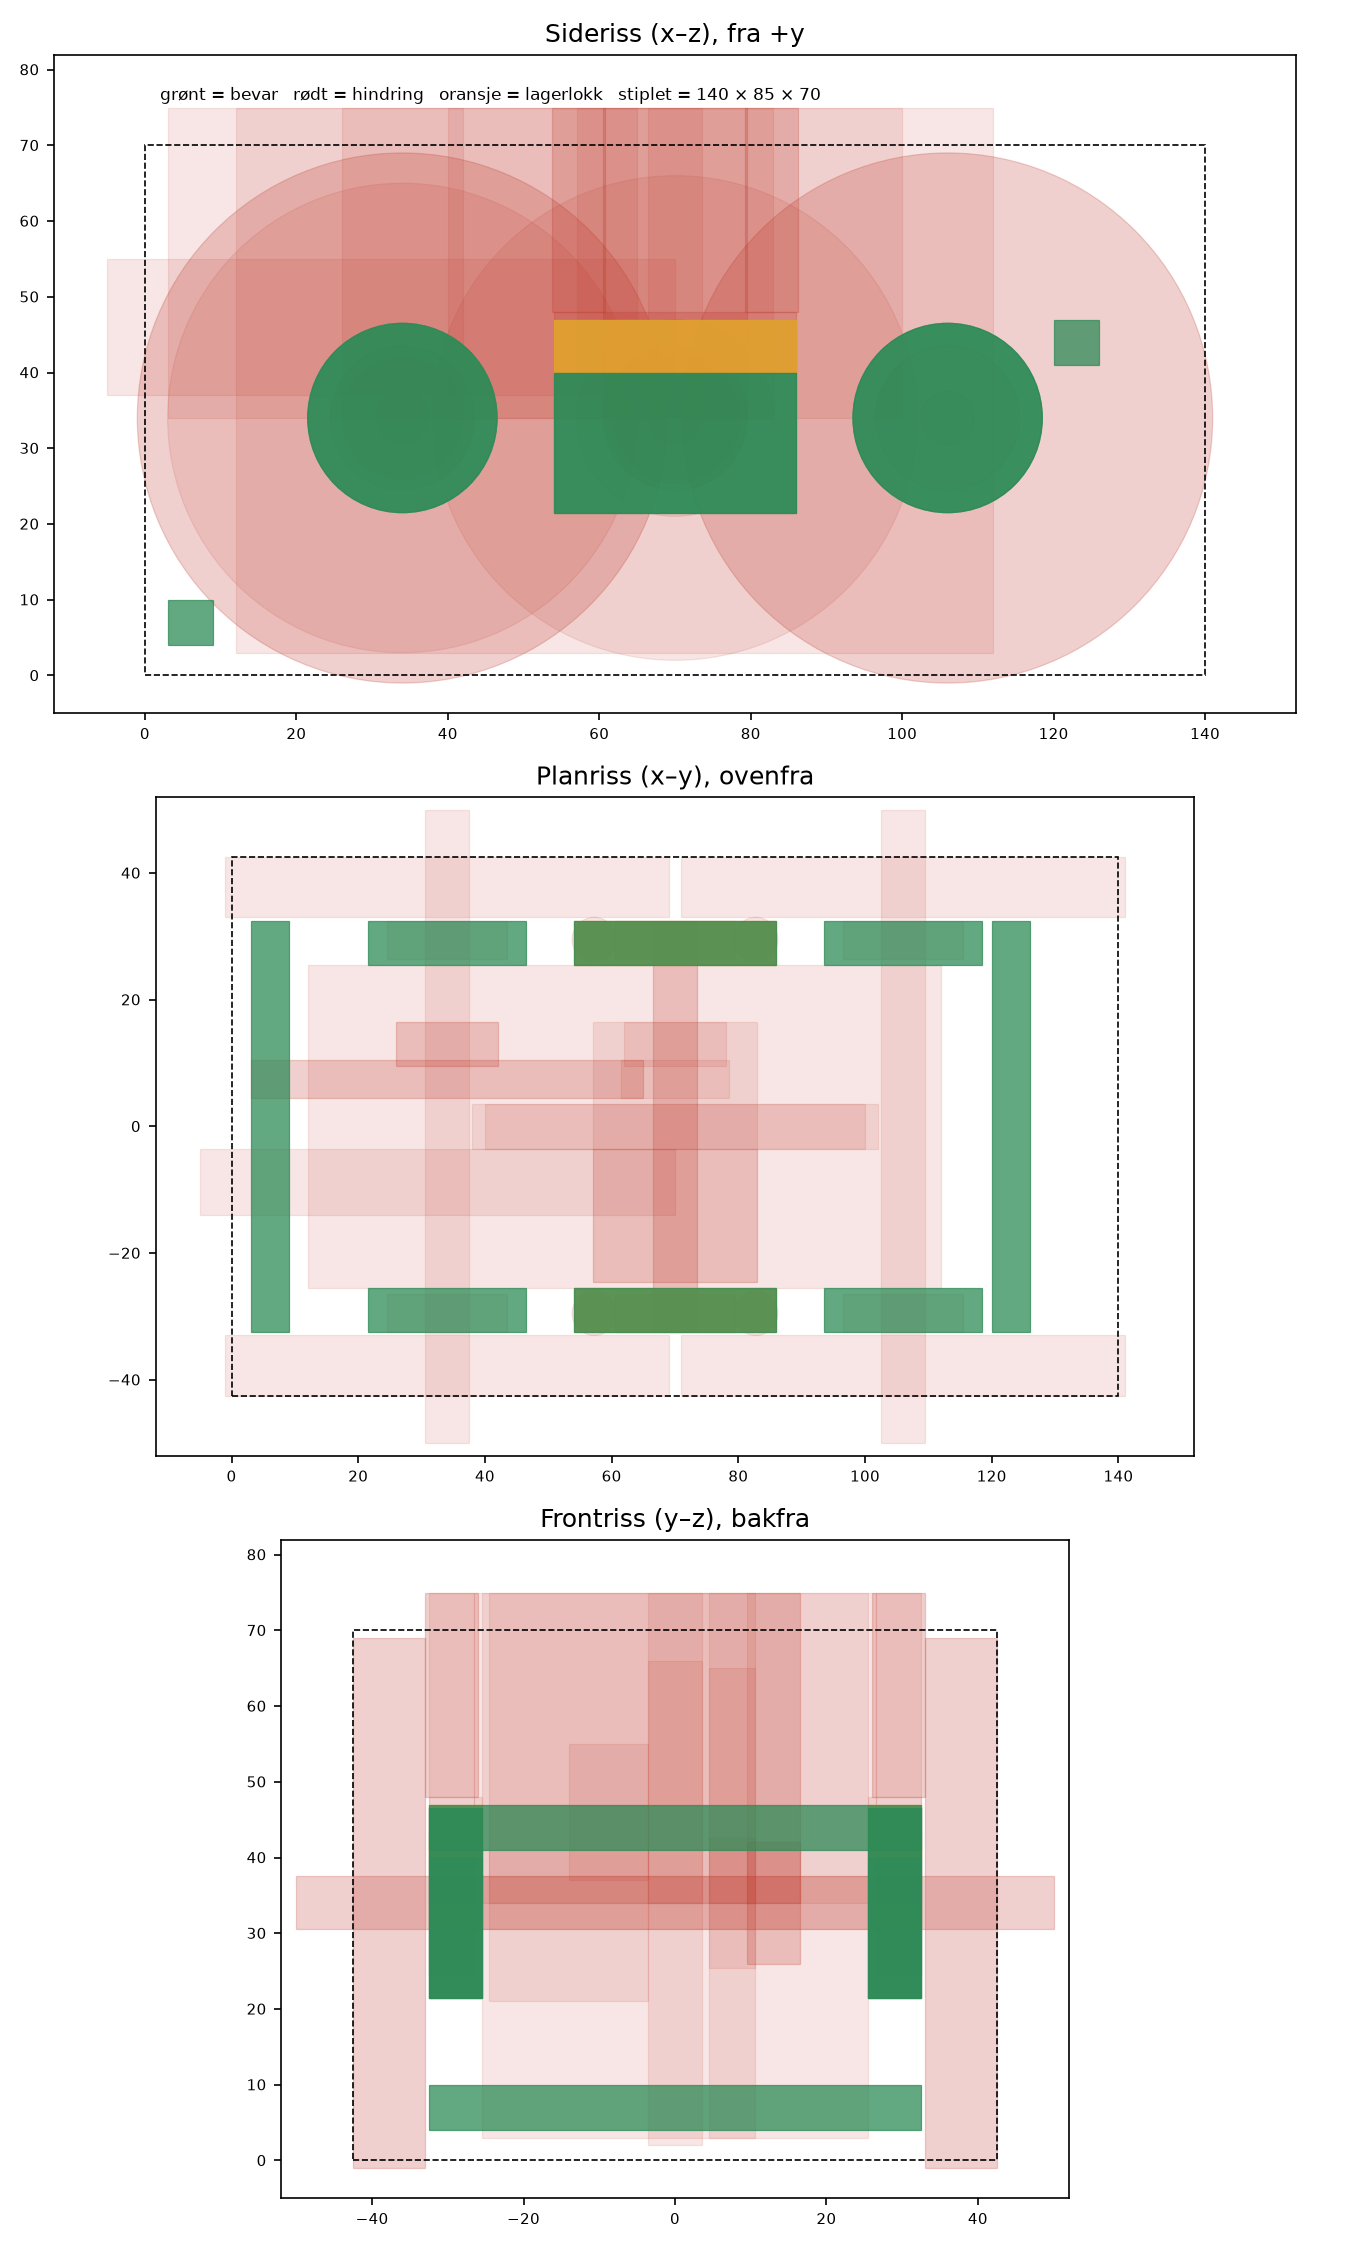
\includegraphics[width=0.48\textwidth]{Images/Ramme/gd_oppsett.png}
    \caption{Oppsettet for generativ design i tre riss. Grønt er bevart geometri, rødt er hindringer, oransje er lagerlokkene og stiplet linje er grensen på $140 \times 85 \times 70$ mm.}
    \label{fig:gd-oppsett}
\end{figure}

\begin{figure}[H]
    \centering
    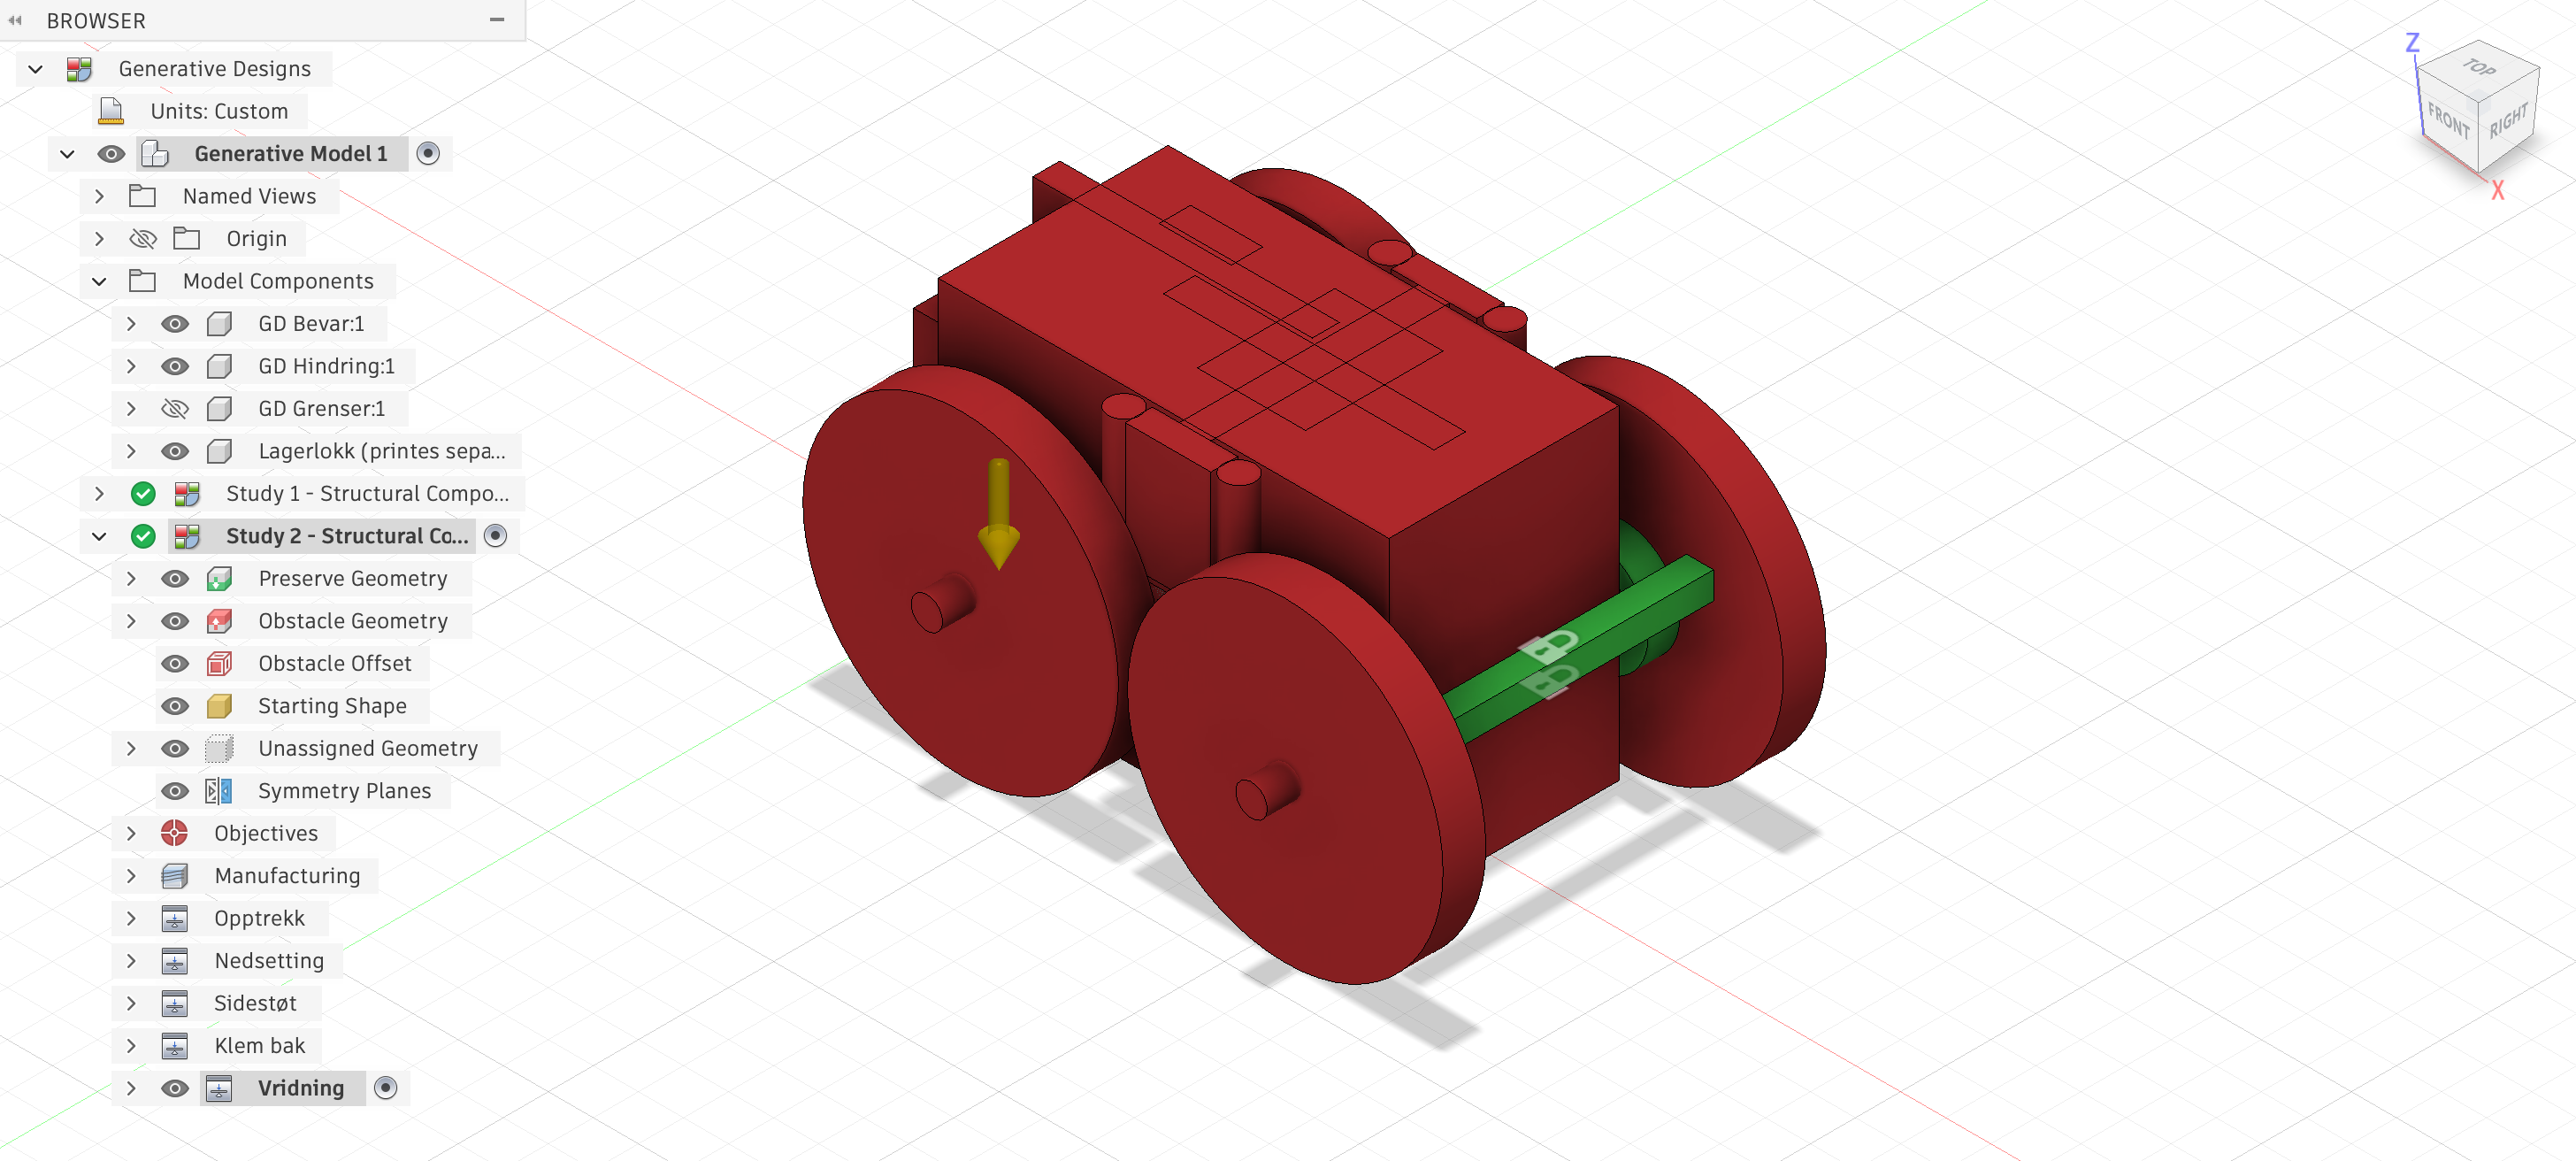
\includegraphics[width=\textwidth]{Images/Ramme/fusion_oppsett.png}
    \caption{Oppsettet i Fusion, med hindringer i rødt og bevart geometri i grønt. Til venstre står de to studiene og de fem lasttilfellene i GD-2. Den gule pila er en av lastene i lasttilfellet for vridning.}
    \label{fig:fusion-oppsett}
\end{figure}

Studien har fem lasttilfeller, vist i tabell~\ref{tab:gd-lasttilfeller}. Snorkraften i opptrekket er satt til \SI{50}{N}, som er det samme som den tidligere gruppen antok \parencite{kers_2026}. Snittkraften i et opptrekk til \SI{4000}{o/min} er omtrent \SI{26}{N} (seksjon~\ref{sec:tr-serien}), så \SI{50}{N} gir margin for toppen i trekket. De andre kreftene er anslått. Ved nedsetting er forakselen fri sideveis. Den tidligere gruppen fant at en ramme som var låst i sideretning, fikk altfor optimistisk stivhet \parencite{kers_2026}.

\begin{table}[H]
    \centering
    \caption{Lasttilfellene i studien for generativ design}
    \label{tab:gd-lasttilfeller}
    \small
    \renewcommand{\arraystretch}{1.3}
    \begin{tabular}{|l|p{4.6cm}|p{5.4cm}|}
        \hline
        \textbf{Lasttilfelle} & \textbf{Innspenning} & \textbf{Last} \\
        \hline
        1. Opptrekk & Fremre tverrbjelke fast & \SI{25}{N} bakover i hvert U-sete \\
        \hline
        2. Nedsetting & Lagerhusene låst, de fremre fri sideveis & \SI{10}{N} nedover i hvert U-sete \\
        \hline
        3. Sidestøt & Som tilfelle 2 & \SI{10}{N} sideveis på fremre tverrbjelke \\
        \hline
        4. Klem bak & Fremre tverrbjelke fast & \SI{20}{N} innover på hvert bakre lagerhus \\
        \hline
        5. Vridning & Fremre tverrbjelke fast & \SI{10}{N} opp på det ene og \SI{10}{N} ned på det andre bakre lagerhuset \\
        \hline
    \end{tabular}
\end{table}

Målet er størst mulig stivhet med et massemål på \SI{40}{g} og sikkerhetsfaktor 2. Fusion har ikke PLA i materialbiblioteket for generativ design, så studien regner med ABS, slik den tidligere gruppen også gjorde. Sikkerhetsfaktoren dekker blant annet at en printet del er svakere mellom lagene enn i lagene. Studien kjøres både uten produksjonsbegrensning og for additiv produksjon. For additiv produksjon er byggeretningen satt langs bilens bredde, slik at rammen printes liggende på siden og lagerboringene blir runde. Største overheng er 45°, og minste godstykkelse er \SI{2}{mm}, som tilsvarer fem perimetre med \SI{0,4}{mm} dyse.

\subsubsection{GD-1: Tre lasttilfeller}
Den første studien hadde bare lasttilfelle 1 til 3. Resultatet var en åpen U-form, der den bakre tverrbjelken bare hang på en tynn stilk (figur~\ref{fig:gd1}). Grunnen var innspenningen. I tilfelle 2 og 3 er begge de bakre lagerhusene låst, og innspenningen virker da som en uendelig stiv bjelke mellom dem. Studien hadde derfor ingen grunn til å bruke materiale på en ekte bjelke bak. En åpen U er lite egnet, fordi den gir etter når bilen holdes bak under opptrekk, og fordi lagrene bak kan vris i forhold til hverandre. Det kan gi en mindre forutsigbar bane.

\begin{figure}[H]
    \centering
    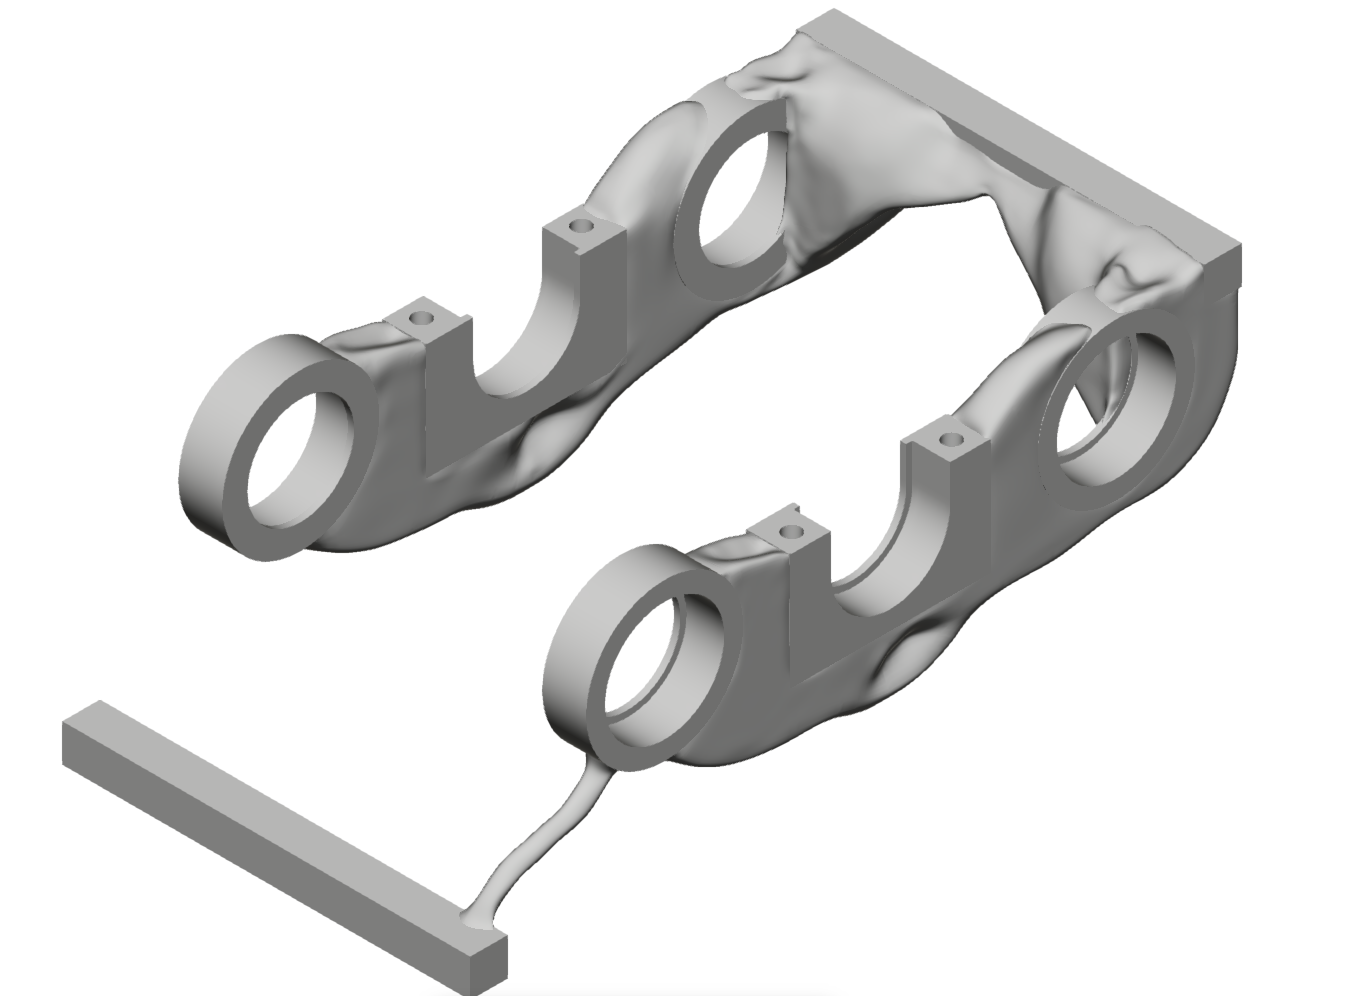
\includegraphics[width=0.55\textwidth]{Images/Ramme/fusion_gd1.png}
    \caption{Resultat 1 fra GD-1, uten produksjonsbegrensning. Uten lasttilfelle 4 og 5 ble rammen en åpen U, der den bakre tverrbjelken (nede til venstre) bare henger på en tynn stilk.}
    \label{fig:gd1}
\end{figure}

\begin{versjonstabell}{GD-1}{tab:gd1}
    \hovedtest
    Lukket ramme rundt drivverket & Mislykket, åpen U \\
    \tilleggstester
    Rammen bærer lastene bak selv & Mislykket, innspenningen tok lastene \\
\end{versjonstabell}

\subsubsection{GD-2: Klem og vridning bak}
\label{sec:gd2}
GD-2 har i tillegg lasttilfelle 4 og 5. Begge holder bare den fremre tverrbjelken fast, så rammen må selv ta opp klemming og vridning bak. Da lønner det seg for studien å lukke rammen.

\begin{figure}[H]
    \centering
    \begin{subfigure}[b]{0.48\textwidth}
        \centering
        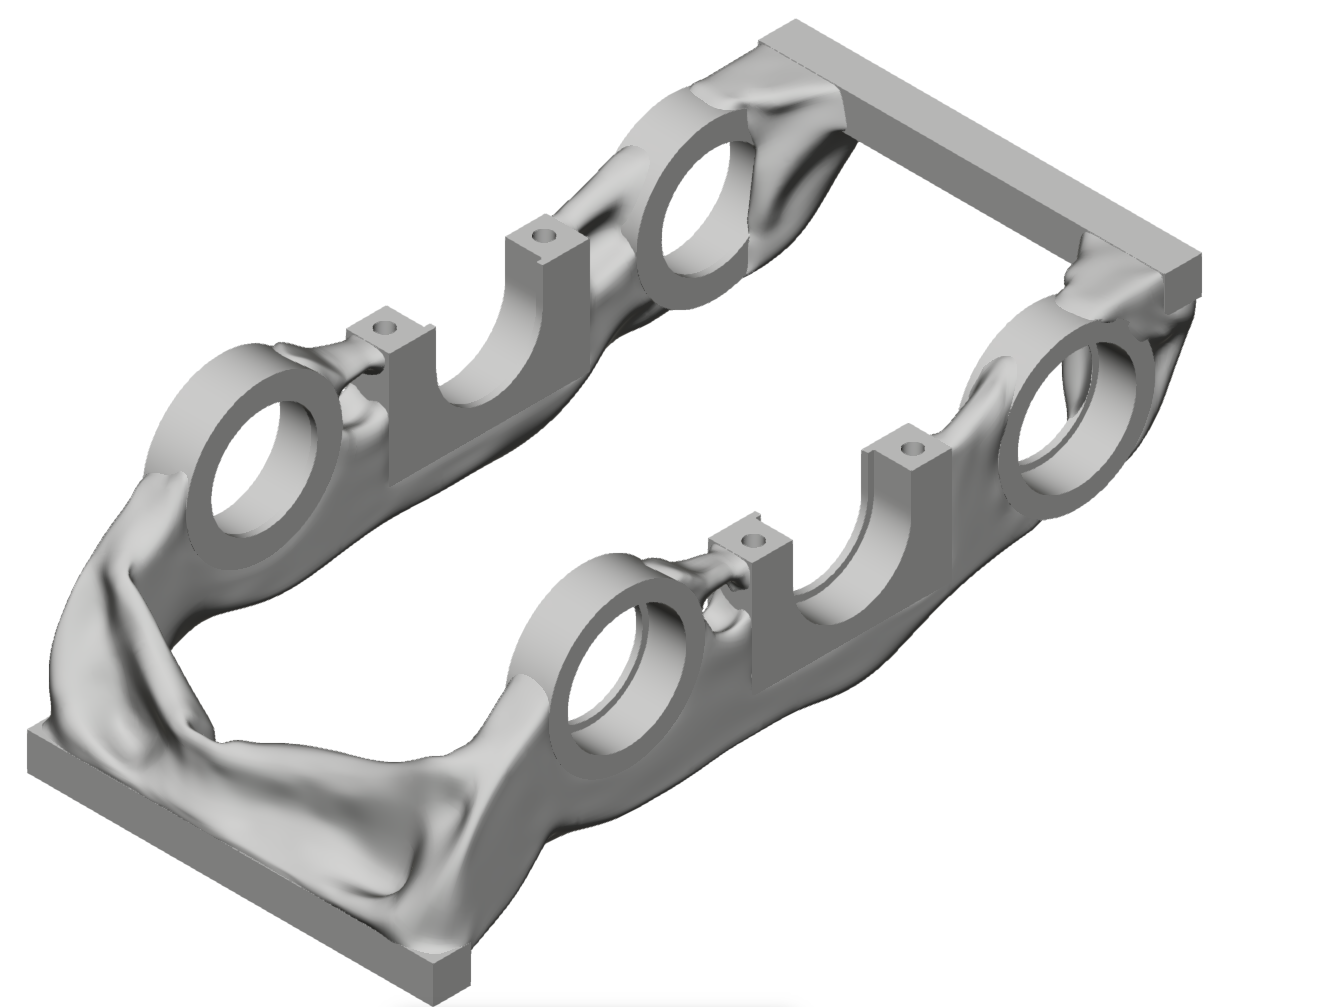
\includegraphics[width=\textwidth]{Images/Ramme/fusion_gd2_utfall1.png}
        \caption{Resultat 1, uten produksjonsbegrensning}
    \end{subfigure}
    \hfill
    \begin{subfigure}[b]{0.48\textwidth}
        \centering
        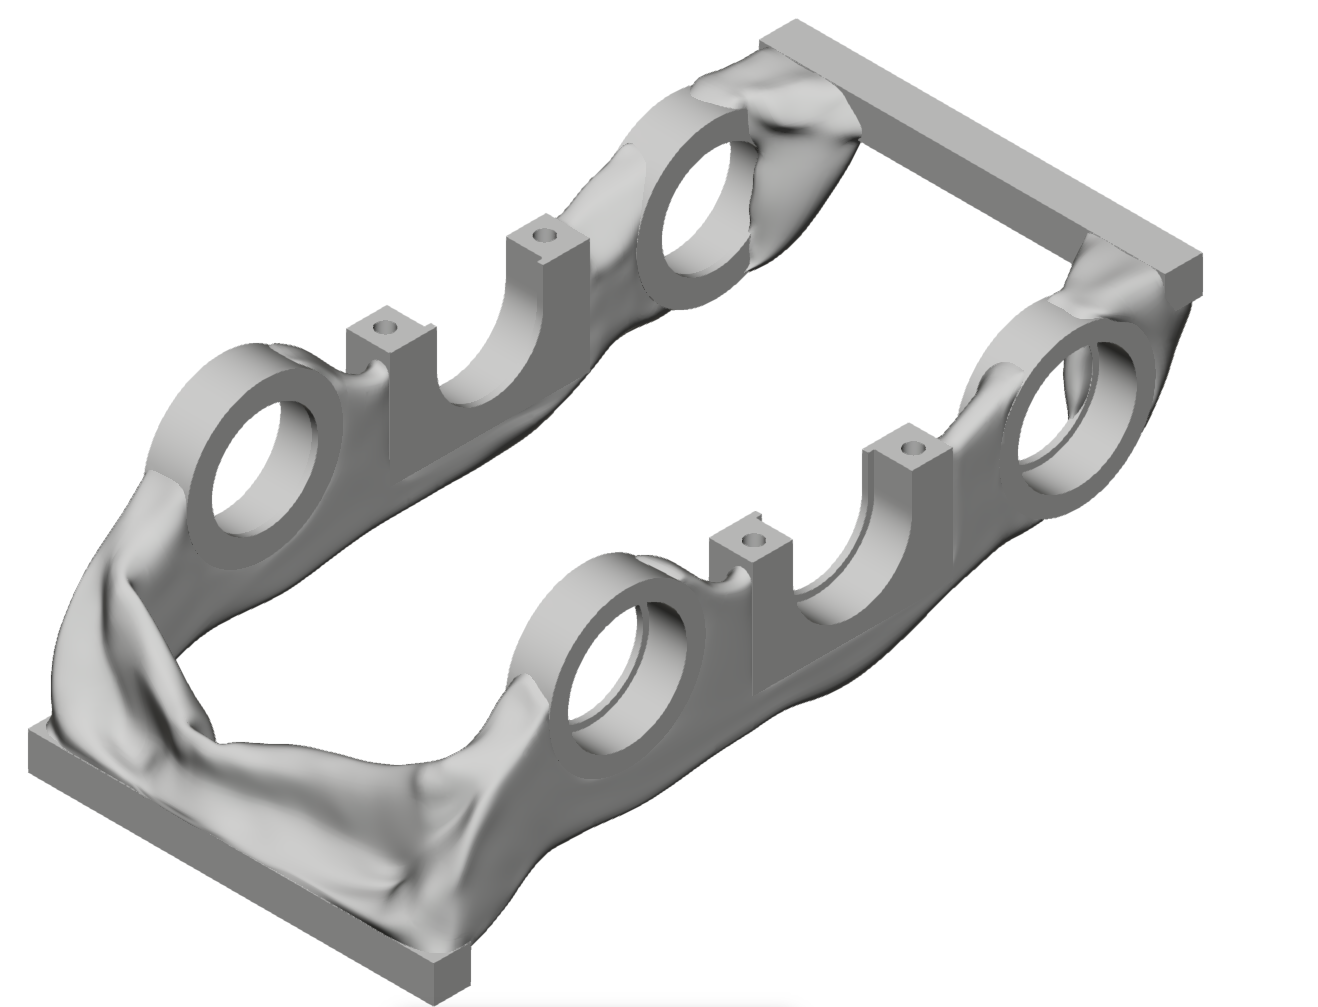
\includegraphics[width=\textwidth]{Images/Ramme/fusion_gd2_utfall2.png}
        \caption{Resultat 2, additiv produksjon (valgt)}
    \end{subfigure}
    \caption{To resultater fra GD-2. Med lasttilfelle 4 og 5 er rammen lukket, og den bakre tverrbjelken er bygd inn i sidene.}
    \label{fig:gd2-utfall}
\end{figure}

Tabell~\ref{tab:gd-resultater} sammenligner resultatene slik Fusion oppgir dem for ABS. Alle tre veier omtrent like mye, fordi massemålet styrer hvor mye materiale studien bruker. Spenningene er svært lave i begge. Den minste sikkerhetsfaktoren i GD-2 er 9,3 til 9,6, langt over kravet på 2. Det er derfor stivheten og minste godstykkelse som bestemmer formen, ikke styrken. GD-2 har dobbelt så høy spenning som GD-1, fordi klem og vridning bak nå bæres av rammen og ikke av innspenningen. Største forskyvning er 0,43 til \SI{0,45}{mm} i alle tre, men GD-1 og GD-2 har ulike lasttilfeller, så tallene kan ikke sammenlignes direkte.

\begin{table}[H]
    \centering
    \caption{Egenskaper for resultatene fra GD-1 og GD-2, regnet i ABS av Fusion}
    \label{tab:gd-resultater}
    \small
    \renewcommand{\arraystretch}{1.3}
    \begin{tabular}{|l|c|c|c|}
        \hline
        \textbf{Egenskap} & \textbf{GD-1, res.~1} & \textbf{GD-2, res.~1} & \textbf{GD-2, res.~2} \\
        \hline
        Produksjon & Fri & Fri & Additiv \\
        \hline
        Form & Åpen U & Lukket & Lukket \\
        \hline
        Volum [\si{cm^3}] & 36,3 & 36,5 & 36,2 \\
        \hline
        Masse i ABS [g] & 38,5 & 38,7 & 38,3 \\
        \hline
        Største von Mises-spenning [MPa] & 1,0 & 2,1 & 2,2 \\
        \hline
        Minste sikkerhetsfaktor & 19,5 & 9,6 & 9,3 \\
        \hline
        Største forskyvning [mm] & 0,44 & 0,43 & 0,45 \\
        \hline
    \end{tabular}
\end{table}

Resultatene er sammenlignet på stivhet, masse og om de er realistiske å printe. Som hos den tidligere gruppen er et robust resultat valgt framfor det letteste \parencite{kers_2026}. Valgt resultat er nummer 2 fra GD-2, vist i figur~\ref{fig:gd2-utfall} og~\ref{fig:gd2-ramme}. Det er laget med begrensningene for additiv produksjon, med byggeretning langs bredden, og så ut til å være det mest printbare. Det har minst uregelmessig geometri mot byggeplaten. Stivheten og sikkerhetsfaktoren er nesten den samme som for resultat 1, så begrensningene for printing koster lite. Rammen måler $123{,}7 \times 65{,}5 \times 43{,}2$ mm. Etter at lagerboringene er utvidet (se under), har den ferdige modellen et volum på \SI{35,8}{cm^3}. I PLA, som er tyngre enn ABS, tilsvarer det omtrent \SI{44}{g} som massiv del. Rammen er printet med \SI{20}{\percent} fyll, og den printede rammen veier \SI{23}{g}. Det er omtrent halvparten av en massiv del. Formen har myke overganger uten skarpe hjørner, der spenningene ellers ville samlet seg.

\begin{figure}[H]
    \centering
    \begin{subfigure}[b]{0.55\textwidth}
        \centering
        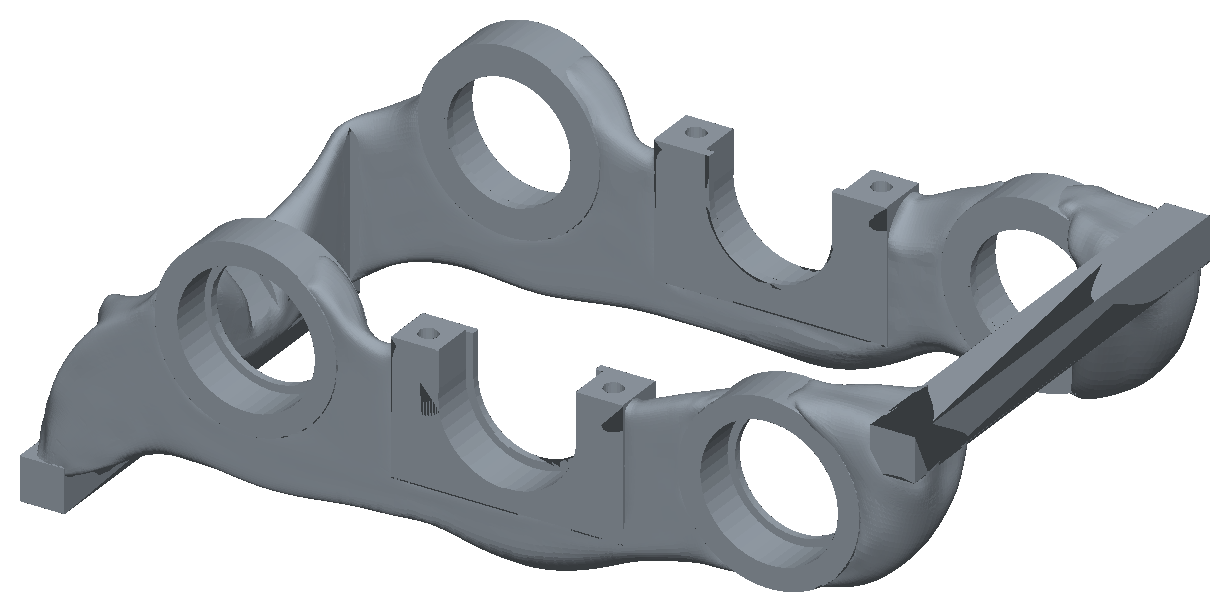
\includegraphics[width=\textwidth]{Images/Ramme/ramme_skraatt.png}
        \caption{Skrått forfra}
    \end{subfigure}
    \hfill
    \begin{subfigure}[b]{0.42\textwidth}
        \centering
        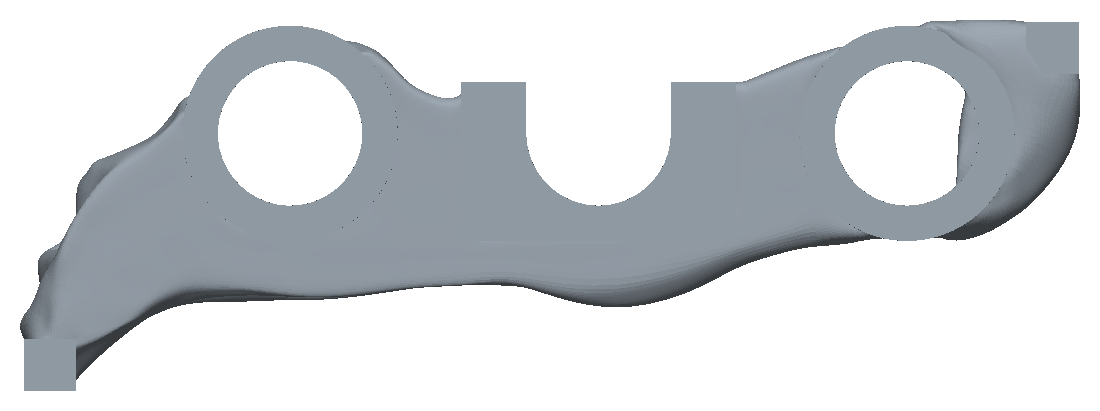
\includegraphics[width=\textwidth]{Images/Ramme/ramme_side.png}
        \caption{Fra siden}
    \end{subfigure}
    \caption{Valgt resultat fra GD-2, slik det ble printet. De fire lagerhusene er lukket, og svinghjulslagrene ligger i U-seter som lukkes med lagerlokk.}
    \label{fig:gd2-ramme}
\end{figure}

\subsubsection{Fra resultat til printet ramme}
Resultatet er gjort om til en vanlig CAD-modell med \emph{Create Design From Outcome}. Den bevarte geometrien beholdes nøyaktig, så lagerboringene blir Ø19,0 som i oppsettet. Prøveringene for lagersetet (seksjon~\ref{sec:ls-serien}) viste at Ø19,0 var stram og Ø19,1 litt romslig. Ø19,1 er valgt, fordi rammen kan slå seg litt under printing og gjøre boringene trangere. Boringene er utvidet i den ferdige modellen i stedet for å kjøre studien på nytt. Før printing ble rammen kontrollert mot drivverket med en kollisjonstest i Fusion, uten treff.

Rammen er printet liggende på siden i PLA på en Bambu Lab H2S med \SI{0,4}{mm} dyse og \SI{20}{\percent} fyll. Den trengte support, selv om studien var satt opp for additiv produksjon med største overheng på 45°. Trolig er grunnen at begrensningen bare gjelder materialet studien legger til. Den bevarte geometrien, som lagerhusene, U-setene og tverrbjelkene, er tegnet uten hensyn til overheng. Fusion-dokumentet sto i centimeter, og den første eksporten som STL ble ti ganger for liten i sliceren. Rammen ble derfor eksportert som 3MF med millimeter som enhet. Lagerlokkene printes for seg og festes med fire M3 × 16-skruer, som skrus rett i Ø2,8-hull i PLA. Godset rundt hullene er bare 1,6 til \SI{1,9}{mm}, så skruene må skrus forsiktig inn første gang, slik at de former gjengene uten at PLA-en sprekker. Gjengeinnsatser fikk ikke plass. Figur~\ref{fig:prototype} viser rammen montert med drivverket.

\begin{versjonstabell}{GD-2}{tab:gd2}
    \hovedtest
    Lukket ramme rundt drivverket & Vellykket \\
    \tilleggstester
    Innenfor $140 \times 85 \times 70$ mm, $123{,}7 \times 65{,}5 \times 43{,}2$ mm (R1) & Vellykket \\
    Ingen kollisjon med drivverket & Vellykket \\
    Svinghjulet kan monteres og tas ut uten å skille rammen (R10) & Vellykket \\
    Masse i ABS \SI{38,3}{g}, massemål \SI{40}{g} & Vellykket \\
    Printet masse \SI{23}{g} med \SI{20}{\percent} fyll & Vellykket \\
    Minste sikkerhetsfaktor 9,3, krav 2 & Vellykket \\
    Kan printes uten support (R13) & Mislykket, trengte support \\
\end{versjonstabell}

\subsubsection{Vurdering}
Kreftene i studien er anslått, bortsett fra at snorkraften er kontrollert mot energien i et opptrekk. Studien regner med massiv ABS, mens rammen er printet i PLA med \SI{20}{\percent} fyll, og en printet del er svakere mellom lagene. Fyllet gjør rammen mindre stiv enn studien regner med. Sikkerhetsfaktoren på 9,3 gir god margin for styrken, men stivheten til den printede rammen er ikke målt. Overhengsbegrensningen i studien var ikke nok til å unngå support, så den bevarte geometrien bør også formes for printing i en senere versjon. Erfaringen fra GD-1 er at innspenningene betyr like mye som lastene: en innspenning som er stivere enn virkeligheten, fjerner behovet for materiale der det trengs. Under testingen viste det seg at svinghjulsakselen hadde for mye klaring sideveis, slik at trommelen kunne komme borti rammen. Det ble løst med avstandshylser og ikke med endringer i rammen (seksjon~\ref{sec:problemlosning}).
